% Introduction
% This chapter aims at understanding the problem.


% Proposed Solution
\section{Proposed Solution}
The solution this thesis proposes is implementing SKFs security expert system to develop secure mobile applications. Each sprint is configured with the level 1 type security verification requirements generated from the MASVS. The following security controls have been included:

\begin{itemize}
    \item \textbf{V1}: Architecture, Design and Threat Modeling Requirements
    \item \textbf{V2}: Data Storage and Privacy Requirements
    \item \textbf{V4}: Authentication and Session Management Requirements
\end{itemize}

\subsection{Security Requirement Analysis}

\subsubsection{Architecture, Design and Threat Modeling Requirements}
CheFeed follows a three-tier software architecture as illustrated in Figure \ref{fig:sys-arch}. Therefore, appropriate security standards must be implemented to all services. The category "Architecture, Design, and Threat Modeling Requirements" ensures that security is addressed when planning the architecture of the mobile app. Table \ref{tab:arch-design-config} describes the sprint configuration for this category. The sprint results described in Table \ref{tab:v1-sprint-results} verification requirements mapped to their MSTG-ID.

\begin{figure}
    \centering
    \caption{System Architecture}
    \label{fig:sys-arch}
    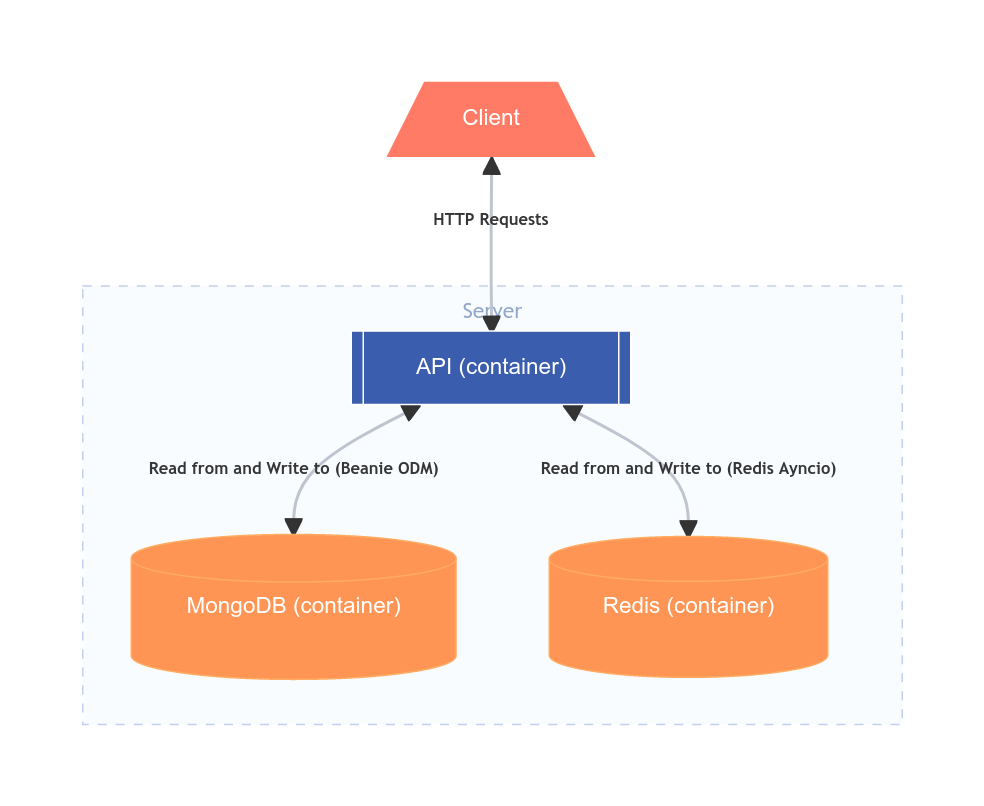
\includegraphics[width=\textwidth]{../../img/chapter-4/system-arch.png}
\end{figure}

\begin{table}
    \centering
    \caption{V1 Sprint Configuration}
    \label{tab:arch-design-config}
    \begin{tabulary}{1.0\textwidth}{|L|L|}
        \hline
        \textbf{Description} & \textbf{Configuration} \\
        \hline
        Centralized security requirements & Yes \\
        \hline
        Does your application accept and process any inputs? & Yes \\
        \hline
        Does your application need to comply with some laws or regulations? & No \\
        \hline
        Does your application need to encrypt data? & Yes \\
        \hline
        Does you application need to have a responsible disclosure policy? & No \\
        \hline
        Update policy requirements & No \\
        \hline
        Does your application need to provide data protection & Yes \\
        \hline
        Secure software development life cycle requirements & Yes \\
        \hline
    \end{tabulary}
\end{table}

\begin{table}
    \caption{Architecture, Design and Threat Modeling Requirements sprint results}
    \label{tab:v1-sprint-results}
    \begin{tabulary}{1.0\textwidth}{|L|L|}
        \hline
        \textbf{MSTG-ID} & \textbf{Description} \\
        \hline
        \textbf{1.1} & All app components are identified and known to be needed \\
        \hline
        \textbf{1.2} & Security controls are never enforced only on the client side, but on the respective remote endpoints \\
        \hline
        \textbf{1.3} & A high-level architecture for mobile app and all connected remote services has been defined and security has been addressed in that architecture \\
        \hline
        \textbf{1.4} & Data considered sensitive in the context of the mobile app is clearly identified \\
        \hline
    \end{tabulary}
\end{table}

\subsubsection{Data Storage and Privacy Requirements}
Personally identifiable information (PII) such as email address or the users full name can be used for identity theft. Therefore, CheFeed must ensure sensitive data is protected. 

\subsubsection{Authentication and Session Management Requirements}
